電気を用いない通信から見てきた通り、通信と記録は密接な関係にある。また、記録の際には記録するべき要素の取捨選択が行われる。人間が直接運ぶにせよ光や音を使うにせよ電気通信にせよ、記録されたものを受け渡しするのが通信であるということに立ち戻れば、記録と通信は表裏一体の関係にあることは明らかであろう。

本章では、離散的な「デジタルデータ」をいかにして表現・記録するかという点について学んでいく。


\section{二元状態とデジタルデータの特徴}

伝言ゲームでは、なかなか情報が正確に伝わらない。この例を見てもわかる通り、通信は記録と伝達手段(伝送路)の双方において正確・確実であり、途中で内容が変化しないことが求められる。

\subsection{記録の条件と二元状態}
記録、すなわち表現において正確性や確実性を担保するためには、次のような条件が必要となろう。
\begin{itemize}
\item いくつかの状態に明確に分かれることあるいは定量的であること。
\item 内容によらず表現方法が統一されていること。
\item 伝送や処理に適した、単純な形態であること。
\end{itemize}

この条件を満たす最も端的な表現として、\textbf{二元状態}\index{にげんじょうたい@二元状態}:明確な二つの状態でそれ以外の状態のないもの があり、実際のデータ伝送において広く用いられている。通信において使われる二元状態は、2進数(0/1)のほか、論理(T/F)、極性(+-)、電流の有無、スイッチのon/offなどが代表的だが、センサの通信などにも目を向ければ動静(動きの有無)、音声(声の有無)なども通信に使われている二元状態といえよう。この二元状態が通信に使われる理由としては、以下のようなものが挙げられる。
\begin{itembox}[l]{二元状態の通信における利点}
\begin{itemize}
\item はっきりと状態の区別がつき、検出も容易で、誤りも生じにくい
\item 多くの電気的状態に一致し、情報の伝送や記憶に有効である
\item 数字の0/1に対応させて2進数表現することで四則・ビット演算を適用できる
\end{itemize}
\end{itembox}

\subsection{デジタルデータの特徴}
デジタルとはよく聞く言葉であるが、この訳語「離散量」あるいは「計数」はそれほど馴染みがない言葉かもしれない。デジタルというのは幾つかの、飛び飛びの状態を取る量という意味であり、対してアナログは連続的に値が定まる。例えば電車の線路が始点からどれだけの距離にあるかはアナログであるが、現在居る駅という情報はデジタルと言える。針が連続に動くアナログ時計は(現実に読み取れるか、その精度はどうかというのは別にして)10.232秒など小数点以下の秒数も表しているが、デジタル時計では数字として表示される桁数以上の情報は捨てられている。

このように、デジタルデータは離散的な有限個の状態に最初からデータが分かれているため、各々に2進数値を対応させることで二元状態の羅列によりデータを表現できる。また、状態が有限個であり、2進数値に対応付けるときに誤差が生じることがない。この例としては、ある文字を音声と書き文字の双方で伝える場合を考えてみよう。文字を音声で伝える際、例えば"し"と"ひ"がごく近い発音だとどちらの文字かひどく伝わりづらいことがある(実際に、江戸言葉や上方言葉ではこれらが混同した発音あるいは入れ替わることがある)。このため、「執事」と「羊」や「しなびた」と「ひなびた」など、"し"と"ひ"しか違いのない2つの言葉は時として文脈などから推定せざるを得ないこととなる。だが、書いている文字であればどちらを指しているのかは一目瞭然であり誤解の恐れはない。ここで挙げたのは極端な例であるが、デジタルデータは最初から状態が明確に分かれていることがアドバンテージとなっているということである。

\subsection{【補足】2進数・記数法について}
\begin{center}
\begin{minipage}[]{0.75\linewidth}
\begin{screen}
\begin{center}
本節は前提知識の補足である。\\
既知の読者におかれては飛ばして次節を読まれたい。
\end{center}
\end{screen}
\end{minipage}
\end{center}

先の解説で2進数を用いたが、記数法について慣れない読者に向け、補足解説を記す。

我々が物を数える際には手の10本の指を用いる。ここから物を数える位取りとして、指がいっぱいになったら位を1増やすということで\textbf{10進法}\index{じっしんほう@10進法}が生まれた。10進法とは、10(十、ten)毎に位がひとつ上がるような数え方であり、我々が普段使っている数の表記法である。10進法により表された数のことを\textbf{10進数}\index{じっしんすう@10進数}と呼ぶ。

一方、先の二元状態は2つの指を持つといえる。そこで、2毎に位がひとつ上がり、0,1,10,11,...と数える\textbf{2進法}\index{にしんほう@2進法}を使う。

これらのような、数の表記にあたりどのようにして位をとるかの方法を\textbf{位取り記数法}\index{くらいどりきすうほう@位取り記数法}(positional notation)あるいは単に\textbf{記数法}\index{きすうほう@記数法}と呼ぶ。また、その位取りの基準となる数(10進法なら10、2進法なら2)を\textbf{基数}\index{きすう@基数}と呼ぶ。

\subsubsection{記数法の一般論}
先までの例と同様に、指の本数から考えよう。指が$n(\ge2)$本しかないと仮定する。このときは、$n$本がいっぱいになったら次の位に移る。たとえば、指が3本しかなければ、3になったら次の位に移るようにして数えることができる。

一般の自然数$n$に対して、$n$進法とは、$n$を基数にする方法である。つまり、数えていって、$n$に達する毎に上の位に移るという事である。

例えば、123という数字を考えよう。これは、123個の1であるが、同時に12個の10と3個の1である。更に分ければ、1個の100と2個の10と3個の1と分かれる。つまり、$10^k$の束がいくつあるかを数え、それが10個に達したら$10^{k+1}$を1増やす。これによって、各位は$10^{k+1}$の束にならない余りとなる。

上記に従って位取りをしてみよう。10進法では、小数点の直上を$10^0$とし、その上の桁を$10^1,10^2,\cdots$、小数点以下を$10^{-1},10^{-2},\cdots$としている。この10を$n$に変えたのが$n$進法である。たとえば、2進法における11111は$2^4\times1+\cdots+2^0\times1=31$である。

$n$進法で使われる数字は、$n$種類ある。2進法なら0と1だし、10進法なら0, 1, 2, 3, 4, 5, 6, 7, 8, 9であり、16進法の場合は0, 1, 2, 3, 4, 5, 6, 7, 8, 9, a, b, c, d, e, fである\footnote{アルファベットは大文字を用いることもある。}。数字だけでは何進法であるかわからない場合もあるため、これを明確にするときには、数字の右下に$33_{(n)}$のように記す。たとえば、$101.1_{(2)}=5.5_{(10)}$である。

\subsubsection{記数法の変換}
$n$進法から10進法への変換はどのように行うだろうか。これは$n$進法の仕組みを考えてみればわかる。

$n^k$の位が$a_k$であるような数字$A$の10進法での値は定義から次のように求められる。
\begin{itembox}[l]{$n$進法から10進法への変換}
$n^k$の位が$a_k$であるような数字$A_{(n)}$は、10進法において
\begin{equation*}
A_{(10)}=\sum_{k}a_k\times n^k
\end{equation*}
と計算できる。
\end{itembox}
逆に、10進法から$n$進法に変える場合は、どうすればよいだろうか。

1つには、単に「取り尽くす」方法がある。つまり、$n^k$のうち、元の数を超えない最大のものを見つけ、その数で元の数を割った商を$n^k$の位にし、余りについて$n^{k-1}$で割り…と繰り返すのである。特に、小数点がある場合はこの方法を利用すると楽である。

だが、この計算はやや面倒に感じることもあろう。そこで、主に整数向けであるが、先に書いた位取りの考えを用いる方法がある。

$n^k$の位が$a_k$であるという事は、$n^k$で割った後に、小数点以下を切り捨て、$n$に対する剰余を取ると$a_k$になる、という事である。例えば、10進法で100の位の数字を出したいとすれば、100で割って10による余りを取れば良い。これと同じ性質が一般の$n$進法にも成立する。この性質を利用し、次のような手順を踏んで記数法を変換できる。
\begin{itembox}[l]{10進法から$n$進法への変換}
\begin{enumerate}
\item 変換したい10進数を$n$で割り、その余りを別におく。
\item これを、商が0になるまで繰り返す。
\item 別においた余りを逆順に並べると$n$進数での表記になる。
\end{enumerate}
\end{itembox}

いくつかの数を変換してみればわかるが、10進整数は他の記数法でも整数である。一方、ある記数法で有限小数であるからと言って他の記数法で有限小数であるとは限らない。例えば、1/3は、10進法では無限小数だが、3進法であれば0.1$_{(3)}$とシンプルに表せる。

\section{情報の符号化}
先にデジタルデータを2進数化して表現することを論じた。情報内容を変えることなく、この2進数化のように用途(記録・通信etc...)に応じて変換を加えることを\textbf{符号化}\index{ふごうか@符号化}あるいは\textbf{エンコード}\index{えんこーど@エンコード}という。必ずしも1/0で表すわけではなく、文字を手旗信号で表すのも符号化の一例といえる。

ここでは整数や文字と言った典型的なデジタルデータの2進数による表現方法(=符号化)を説明する。また、やや歴史的な符号化の例としてモールス符号を、デジタルでアナログを近似している例として小数の表現方法を紹介する。

なお、これ以降の議論については、二元状態として\textbf{bit}\index{bit}(binary digitの略で二進数の意)を用いるものとし、8bitである場合の表現として1\textbf{byte(バイト)}\index{byte}あるいは(歴史的経緯により)特に8bitであることを強調したい際には1\textbf{octet(オクテット)}\index{octet}を用いる\footnote{2008年まで、1byte=8bitであることは主流でこそあったものの明確な定義として定まっておらず、1byteが8bitでない環境も存在していた。2008年にISO(国際標準化機構)やIEC(国際電気標準会議)において1byte=1octetが正式に定まったため、現在では1byte=8bitとして考えて問題はないが、追随できていない環境などでは1byteが8bitでない可能性もありうる。このことから、本書においては8bitであることが特に重要な場合には旧来の1octetという表記を用いることとした。}。

\subsection{整数の表現}
2進数での表現として最も単純なのは符号なし整数であろう。符号なしの整数をそのまま2進数に変換し、これをビットパターンとする方法である。$N$bitにより、0以上$2^{N}$未満の整数が表現される。

一方、符号付き整数を扱う場合にはどうだろうか。例えば、先頭の1ビットを符号に割り当てるなどの方法が考えられる。だが、この方法では+0と-0が出る、符号の扱いの都合でCPUの実装等が複雑になるなどの難点がある。これらの理由の回避のため、近年の電子計算機では\textbf{2の補数}\index{2のほすう@2の補数}表現が用いられることが多い。

この表現は、次のようなものである。

まず、0を基準とする。10進法における0を、2進法における0と対応させるのは自然な考えであろう。さて、これから1を引いた数、すなわち-1をどう表すべきであろうか??

4ビットで考えることとしよう。1=0001から1を引くと0=0000になる。では、それより1小さいものはどうすればいいか。これは、1111とすれば良いのである。ビットがあふれる部分への繰り上がりあるいはその部分からの繰り下がりを無視して考えれば、0000-1=1111であるし、足し算で考えても1111+0001=0000, 0000+0001=0001となる。また、嬉しいことに、この方法を用いた場合でも、先頭ビット0は+または符号なしを、1は-を示す。このように、-aのビット表現を、0からaを引いたものとして表現するのが2の補数表現である。

参考として、表\ref{table1_1}に、2の補数表現を用いた4ビットの場合の符号なし整数・符号あり整数一覧を示す。
\begin{table}[htb]
\centering
\caption{4bit符号なし整数・符号あり整数の一覧}\label{table1_1}
\begin{tabular}{|c|c|c||c|c|c|}\hline
ビット列&符号なし整数&符号あり整数&ビット列&符号なし整数&符号あり整数\\ \hline
&&&&&\\[-16pt]\hline
0000&0&0&1000&8&-8\\ \hline
0001&1&1&1001&9&-7\\ \hline
0010&2&2&1010&10&-6\\ \hline
0011&3&3&1011&11&-5\\ \hline
0100&4&4&1100&12&-4\\ \hline
0101&5&5&1101&13&-3\\ \hline
0110&6&6&1110&14&-2\\ \hline
0111&7&7&1111&15&-1\\ \hline
\end{tabular}
\end{table}

この例を見てもわかるように、(桁溢れの繰り上がりを無視すれば)2進数・10進数とも順に並んでいるのが2の補数表現の特徴である。また、符号を用いた表現と違い0が1つになっており、-8から7までと、負の側は絶対値が1大きい値まで収まる。

\subsubsection{【補遺】補数の意味}
\begin{center}
\begin{minipage}[]{0.75\linewidth}
\begin{screen}
\begin{center}
本節は大筋に影響しない。\\
難解あるいは興味索然たるものと感じる折には\\
飛ばして次節を読まれたい。
\end{center}
\end{screen}
\end{minipage}
\end{center}

先の解説では2の補数表現について補数とは何か説明せずに仕組みのみを述べた。本節では、関心ある読者諸賢に向け、\textbf{補数}\index{ほすう@補数}の意味について解説する。

ある基数$b$における自然数$a$の補数とは、$a$に足した時に桁が1増えるような最小の自然数$c$のことをいう\footnote{厳密にはこの$c$を($b$進法における)基数の補数($b$の補数)と、$c$を1小さくしたものを($b$進法における)減基数の補数($b-1$の補数)と呼ぶ。本書で出てくるのは全て前者である}。10進法における74に対する補数は26である。2進数において$1100_{(2)}=12_{(10)}$の補数は$100_{(2)}=4_{(10)}$である。

先に出てきた2の補数表現とは、2進数における$a$の補数を$-a$として使う($a>0$)という考えである。但し、一般の補数では直上の1桁が増えるかどうか見るところ、この表現においては扱うサイズで桁溢れが起きるかどうかにより判断をする。換言すれば、「符号なし整数の最大値+1から$a$を引いた値」といえる。先に挙げた4bitにおける5(0101)の補数は、4bitが桁溢れを起こすような最小の自然数、つまり16(10000)-5(0101)=11(1011)である。そこで、1011という表現を-5の表現とする。同じように、$a$の補数の符号なし整数表現(2進数表現)を$-a$として使う($a>0$)というのが、2の補数表現である。


\subsection{文字の表現}
デジタルデータとして文字を表現する場合には、それぞれの2進数値に対応した文字を定める。これを\textbf{文字コード}\index{もじこーど@文字コード}と呼ぶ。例えば、最も一般的な文字コードと言えるASCII(American Standard Code for Information Interchange)の場合、数字の9は57となり、文字Aは65に割り当てられている(表\ref{table1_2})。ここではASCIIの例を出したが、文字コードには様々な種類があり、それによって同じ数字でも違う文字に割り当てられることがある。
\begin{table}
\centering
\caption{ASCIIコード一覧(16進接頭辞0xは省いた)}\label{table1_2}
\begin{tabular}{|c|c|c||c|c|c||c|c|c|}\hline
10進&16進&文字&10進&16進&文字&10進&16進&文字 \\ \hline
 & & &&&& & & \\[-15pt] \hline
0&00&\verb|NUL|{\scriptsize (null文字)}&16&10&\verb|DLE|{\scriptsize (伝送制御拡張)}&32&20&(空白)\\ \hline
1&01&\verb|SOH|{\scriptsize (ヘッダ開始)}&17&11&\verb|DC1|{\scriptsize (装置制御1)}&33&21&\verb|!|\\ \hline
2&02&\verb|STX|{\scriptsize (テキスト開始)}&18&12&\verb|DC2|{\scriptsize (装置制御2)}&34&22&\verb|"|\\ \hline
3&03&\verb|ETX|{\scriptsize (テキスト終了)}&19&13&\verb|DC3|{\scriptsize (装置制御3)}&35&23&\verb|#|\\ \hline
4&04&\verb|EOT|{\scriptsize (転送終了)}&20&14&\verb|DC4|{\scriptsize (装置制御4)}&36&24&\verb|$|\\ \hline
5&05&\verb|ENQ|{\scriptsize (照会)}&21&15&\verb|NAK|{\scriptsize (受信失敗)}&37&25&\verb|%|\\ \hline
6&06&\verb|ACK|{\scriptsize (受信OK)}&22&16&\verb|SYN|{\scriptsize (同期)}&38&26&\verb|&|\\ \hline
7&07&\verb|BEL|{\scriptsize (警告)}&23&17&\verb|ETB|{\scriptsize (転送ブロック終了)}&39&27&\verb|'|\\ \hline
8&08&\verb|BS|{\scriptsize (後退)}&24&18&\verb|CAN|{\scriptsize (とりけし)}&40&28&\verb|(|\\ \hline
9&09&\verb|HT|{\scriptsize (水平タブ)}&25&19&\verb|EM|{\scriptsize (メディア終了)}&41&29&\verb|)|\\ \hline
10&0a&\verb|LF|{\scriptsize (改行)}&26&1a&\verb|SUB|{\scriptsize (置換)}&42&2a&\verb|*|\\ \hline
11&0b&\verb|VT|{\scriptsize (垂直タブ)}&27&1b&\verb|ESC|{\scriptsize (エスケープ)}&43&2b&\verb|+|\\ \hline
12&0c&\verb|FF|{\scriptsize (改頁)}&28&1c&\verb|FS|{\scriptsize (フォーム区切り)}&44&2c&\verb|,|\\ \hline
13&0d&\verb|CR|{\scriptsize (復帰)}&29&1d&\verb|GS|{\scriptsize (グループ区切り)}&45&2d&\verb|-|\\ \hline
14&0e&\verb|SO|{\scriptsize (シフトアウト)}&30&1e&\verb|RS|{\scriptsize (レコード区切り)}&46&2e&\verb|.|\\ \hline
15&0f&\verb|SI|{\scriptsize (シフトイン)}&31&1f&\verb|US|{\scriptsize (ユニット区切り)}&47&2f&\verb|/|\\ \hline
\end{tabular}
 \newline
\centering
\begin{tabular}{|c|c|c||c|c|c||c|c|c||c|c|c|}\hline
10進&16進&文字&10進&16進&文字&10進&16進&文字&10進&16進&文字\\ \hline
& & & & & & & & & & & \\[-15pt] \hline
48&30&\verb|0|&68&44&\verb|D|&88&58&\verb|X|&108&6c&\verb|l|\\ \hline
49&31&\verb|1|&69&45&\verb|E|&89&59&\verb|Y|&109&6d&\verb|m|\\ \hline
50&32&\verb|2|&70&46&\verb|F|&90&5a&\verb|Z|&110&6e&\verb|n|\\ \hline
51&33&\verb|3|&71&47&\verb|G|&91&5b&\verb|[|&111&6f&\verb|o|\\ \hline
52&34&\verb|4|&72&48&\verb|H|&92&5c&\verb|\|&112&70&\verb|p|\\ \hline
53&35&\verb|5|&73&49&\verb|I|&93&5d&\verb|]|&113&71&\verb|q|\\ \hline
54&36&\verb|6|&74&4a&\verb|J|&94&5e&\verb|^|&114&72&\verb|r|\\ \hline
55&37&\verb|7|&75&4b&\verb|K|&95&5f&\verb|_|&115&73&\verb|s|\\ \hline
56&38&\verb|8|&76&4c&\verb|L|&96&60&\verb|`|&116&74&\verb|t|\\ \hline
57&39&\verb|9|&77&4d&\verb|M|&97&61&\verb|a|&117&75&\verb|u|\\ \hline
58&3a&\verb|:|&78&4e&\verb|N|&98&62&\verb|b|&118&76&\verb|v|\\ \hline
59&3b&\verb|;|&79&4f&\verb|O|&99&63&\verb|c|&119&77&\verb|w|\\ \hline
60&3c&\verb|<|&80&50&\verb|P|&100&64&\verb|d|&120&78&\verb|x|\\ \hline
61&3d&\verb|=|&81&51&\verb|Q|&101&65&\verb|e|&121&79&\verb|y|\\ \hline
62&3e&\verb|>|&82&52&\verb|R|&102&66&\verb|f|&122&7a&\verb|z|\\ \hline
63&3f&\verb|?|&83&53&\verb|S|&103&67&\verb|g|&123&7b&\verb|{|\\ \hline
64&40&\verb|@|&84&54&\verb|T|&104&68&\verb|h|&124&7c&\verb`|`\\ \hline
65&41&\verb|A|&85&55&\verb|U|&105&69&\verb|i|&125&7d&\verb|}|\\ \hline
66&42&\verb|B|&86&56&\verb|V|&106&6a&\verb|j|&126&7e&\verb|~|\\ \hline
67&43&\verb|C|&87&57&\verb|W|&107&6b&\verb|k|&127&7f&\verb|DEL|{\scriptsize (削除)}\\ \hline
\end{tabular}
\end{table}

1オクテットでは256通りの文字しか表わせないため、日本ではひらがな・カタカナ・漢字を表すのに不十分である。そのため、日本語を扱う際などには、それらにも対応したShift\_JISやEUC-JP(Extended UNIX Code Packed Format for Japanese)、UTF-8などの日本語の文字コードを使うことになる。Webページなどを閲覧している時に文字化けして見えることがあるが、この多くは異なる文字コードを使っていることによるものである。異なる文字コードであれば当然違う文字が割り当てられているため、本来と違うコードによって解釈されてしまうと意図した文字と異なる文字として扱われるということである。

\subsection{モールス符号}
文字列の符号化として多くの制御文字があるASCIIより歴史ある例として、\textbf{モールス符号}\index{もーるすふごう@モールス符号}があげられる。これは短点(\verb|・|。日本語ではトンと呼ばれる)と長点(\verb|-|。同じく日本語ではツーと呼ばれる)の2元状態を用いた符号である。英文中の発生頻度の高いアルファベットには短い符号、発生頻度の低いアルファベットには比較的長い符号を割り当てることで、平均的な符号長を短縮したものである(表\ref{table1_3}参照)。

\begin{table}[htbp]
\centering
\caption{国際モールス符号のアルファベット}\label{table1_3}
\begin{tabular}{|c|c|c||c|c|c||c|c|c|}\hline
英字&出現率&符号&英字&出現率&符号&英字&出現率&符号\\ \hline  
&&&&&&&& \\[-15pt] \hline
A&6.42\%&\verb|・-|&J&\underline{0.08\%}&\verb|・---|&S&5.14\%&\verb|・・・|\\ \hline
B&1.27\%&\verb|-・・・|&K&0.49\%&\verb|-・-|&T&\textbf{7.96\%}&\verb|-|\\ \hline
C&2.18\%&\verb|-・-・|&L&3.21\%&\verb|・-・・|&U&2.28\%&\verb|・・-|\\ \hline	
D&3.17\%&\verb|-・・|&M&1.98\%&\verb|--|&V&0.83\%&\verb|・・・-|\\ \hline			
E&\textbf{10.31\%}&\verb|・|&N&5.74\%&\verb|-・|&W&1.75\%&\verb|・--|\\ \hline	
F&2.08\%&\verb|・・-・|&O&6.32\%&\verb|---|&X&0.13\%&\verb|-・・-|\\ \hline
G&1.52\%&\verb|--・|&P&1.52\%&\verb|・--・|&Y&1.64\%&\verb|-・--|\\ \hline
H&4.67\%&\verb|・・・・|&Q&\underline{0.08\%}&\verb|--・-|&Z&\underline{0.05\%}&\verb|--・・|\\ \hline
I&5.75\%&\verb|・・|&R&4.84\%&\verb|・-・|&空白&\textbf{18.59\%}&\\ \hline
\end{tabular}
\end{table}

長点は短点の3倍の長さと定まっており、また点と点の間には短点1つ分の間隔を空ける。文字間隔は短点3つ分、語間隔は短点7つ分と定められている。

\subsection{小数の表現}
小数は(無限小数なども含めれば)文字や整数と違い、連続的な(アナログな)データである。このため、先に挙げたデジタルデータの利点である「元から離散的で有限個」という性質がなく、デジタル表現のために「最も近い表現可能な値」に丸める必要がある。これは次章のアナログデータの表現で出てくる量子化というステップであり、これによる誤差(プログラミングの世界では一般に丸め誤差という)は量子化雑音に相当する。

コンピュータ等で扱う小数は、数学等の小数と違い、表せる個数が限られたデジタルデータである。本来はアナログデータである小数を出来る限り近い値で表せるように考えられたデジタル表現とも言える。その表現方法には\textbf{固定小数点数表現}\index{こていしょうすうてんすうひょうげん@固定小数点数表現}と\textbf{浮動小数点数表現}\index{ふどうしょうすうてんすうひょうげん@浮動小数点数表現}がある\footnote{それぞれ、固定-小数点-数、浮動-小数点-数と区切る。対応する英語も、fixed point number,floating point numberである。}。

\subsubsection{固定小数点数}
ある定まったビットまでを整数部として、そこから下の部を小数部としてみなすことでしょうすうを表現する方法を、固定小数点数表現\index{こていしょうすうてんすうひょうげん@固定小数点数表現}という。例えば、16ビットある時に、上位8ビットがその数の整数部を示し、下位8ビットが小数部を示すようにすれば良い。この時、$2^0=1$を示すビットのすぐ下のビットは$2^{-1}$を、その下は$2^{-2}$を$\cdots$というように、桁が連続的に定まっていくのが普通である。

この方式は表現できる数の範囲はごく限られるものの(例えば先の16bitの例ならば、10進数で1/256刻みの値しか扱えない)、定められた範囲においては、誤差を出すことなく高速に計算できる。10の累乗で表現するような値が頻出する科学計算では利用しづらいが、桁数がある程度定まっている上に誤差が大きな問題となる経済計算などで用いられる。

\subsubsection{浮動小数点数}
浮動小数点数表現\index{ふどうしょうすうてんすうひょうげん@浮動小数点数表現}は、小数点の場所を上手く変えながら(浮動)表す方法である。浮動小数点数では、表したい数をまず以下の形式で表現する。
\[\text{(符号)}\text{(仮数)}\times\text{(基数)}^\text{(指数)}\]
この内、基数は通常2が用いられる。また、仮数は1以上2未満の数である(これにより、上記の形式での表現が一意に定まる)。そして、符号(1bit)、指数(符号付き整数)、仮数の小数部(固定小数点数)を各々保存する。例えば、-4.8という数字を浮動小数点数で表現することを考えよう。$-4.8=-1.2\times 2^2$である。したがって、符号部には-が、仮数部には0.2が、指数部には2が格納されることになる。なお、指数・仮数を何bitとするかは規格によって異なるが、近年のコンピュータではIEEE754という規格に従っていることが多い。

固定小数点数型に比べ、指数部の表現によって科学計算などで用いるような大小様々な値に比較的近い値を表現できるが、誤差が出たり、計算の時間がかかったりといった問題点もある。固定小数点数型は狭い範囲を等間隔に区切っている表現であるが、浮動小数点数は広い範囲をその絶対値に応じてスケーリングして区切っているという見方もできる。


\section{符号化効率の改善と圧縮}
データの記録や通信の資源は限られているため、少しでも効率よく記録・通信したい。先に挙げたモールス信号は光あるいは音を人間が認識して行うことから伝達に時間がかかる。そのため、少しでも短縮するために文字の出現頻度を考慮して符号の長さが決まっていた。同様に、何らかの手法を用いてデータを\textbf{圧縮}\index{あっしゅく@圧縮}して符号化する、あるいは符号化したものを圧縮する方法が考えられた。

\subsection{符号化効率の改善}
先に扱った例では、取りうる値各々に定長を割当てて情報を表していた。しかし、何らかの手法でこの定長を短くしたり、可変長にしたりすることで、同じ情報でもより短い符号にて記録できる。

サイコロの出目を考えよう。6つの面が等確率で出る普通のサイコロの場合、単に定長を割り当てるなら3bitが必要になる。しかし、00,01,100,101,110,111と言う6通りの状態を出目に対応させると、\textbf{平均符号長}\index{へいきんふごうちょう@平均符号長}は
\[\frac{1}{6}\text{(の確率)}\times 2\text{(bit)} \times 2\text{(通り)}+\frac{1}{6}\text{(の確率)}\times 3\text{(bit)} \times 4\text{(通り)}=\frac{8}{3}\]
となり、3bitの定長で割り当てる場合に比べておよそ11\%短いデータで表現できている。また、ここで表した6つの符号は「先頭から読む際、0を読んだら2bit,1を読んだら3bit」というルールを課すことで混同することなく元の情報を取り出すことができる。

このように、データ量を節約することは保存の上でも無論便利であるが、より短時間での通信や記録が可能となるため利便性が大きい。

\subsubsection{モールス符号の平均符号長}
モールス符号は文字の出現頻度を考慮して符号の長さが決まっていたと記したが、実際の平均符号長はどのぐらいか計算してみよう。表\ref{table1_4}に各符号の符号長(符号の文字数)と、その点長(一つの文字を表すのにかかるのが短点の何倍になるか)を記した。

\begin{table}[htbp]
\centering
\caption{国際モールス符号の英字符号長}\label{table1_4}
\begin{tabular}{|c|c|c|c||c|c|c|c||c|c|c|c|}\hline
英字&出現率&語長&点長&英字&出現率&語長&点長&英字&出現率&語長&点長\\ \hline
&&&&&&&&&&& \\[-15pt] \hline
A&6.42\%&2&6&J&0.08\%&4&13&S&5.14\%&3&5\\ \hline
B&1.27\%&4&9&K&0.49\%&3&9&T&7.96\%&1&3\\ \hline
C&2.18\%&4&11&L&3.21\%&4&9&U&2.28\%&4&7\\ \hline
D&3.17\%&3&7&M&1.98\%&2&7&V&0.83\%&7&9\\ \hline
E&10.31\%&1&1&N&5.74\%&2&5&W&1.75\%&4&9\\ \hline
F&2.08\%&4&9&O&6.32\%&3&11&X&0.13\%&4&12\\ \hline
G&1.52\%&3&9&P&1.52\%&4&11&Y&1.64\%&4&13\\ \hline
H&4.67\%&4&7&Q&0.08\%&4&13&Z&0.05\%&4&11\\ \hline
I&5.75\%&2&3&R&4.84\%&3&7&空白&18.59\%&0&1\\ \hline
\end{tabular}
\end{table}

ここで、点長は、長点が短点の3倍の長さで、点と点の間が1倍の長さであることから、長点の数$\times 3+$短点の数(空白も含む)$+$文字数$-1$で計算している(実際には、これに字間・語間の長さが加わるが、これは無視している)。

表\ref{table1_4}を元に、平均符号長を計算する。出現率$\times$語長の総和を取ると、2.12となり、空白を込めて27通りのデータであるにもかかわらず、二元状態2文字強とかなり短くなっていることがわかる。また、同様に各文字の点長の平均は(短点を1として)5.18の長さである。仮に文字を全て固定長5bitにし1を長点・0を短点・字間の空白は同じと考えると、(最も効率よく当てはめたとしても)2倍以上の長さとなるため、長さを2元状態にするという制約下においてモールス符号は効率化されていることがわかるだろう\footnote{但し、モールス符号は最適な割り当て方をしているとは言えない。平均符号長を最適化すると1.99となってその時の点長の平均は4.95と5を切る。点長の平均を最適化した場合は4.84となり、平均符号長は2.07と、より良い方法もある点には留意されたい。}。


\subsection{可逆圧縮・不可逆圧縮}
圧縮には大きく分けて、「本来の情報のうち不要な部分を捨て去ることにより符号を短くする」手法と、「本来の情報の何らかの特性を利用してより短い表現を用意し符号を短くする」手法がある。前者のように、元の情報から何らかの情報が捨てられるケースでは捨て去られた部分のデータを復元して元のデータに戻すことは不可能であるので、\textbf{不可逆圧縮}\index{ふかぎゃくあっしゅく@不可逆圧縮}(あるいは\textbf{非可逆圧縮}\index{ひかぎゃくあっしゅく@非可逆圧縮}と呼ばれる。一方、後者の手法は元のデータに戻すことが可能なので\textbf{可逆圧縮}\index{かぎゃくあっしゅく@可逆圧縮}と呼ばれる。本来の圧縮の手法では元のデータの復元が可能であることが条件なので不可逆圧縮は圧縮とは呼べないともされるが、現実的には圧縮の一種として扱われている。

電気を使わない世界での不可逆圧縮の例を考えてみよう。不可逆圧縮としては、電車の遅延証明書が挙げられる。電車の遅延証明書は「この時間帯に最大で○分の遅れが出たことを証明する」と言う形式になっている。それぞれの電車についてどの駅で何分遅れたかは、データとしては存在するだろう。しかし、そのような細かい情報は遅延証明書を必要とする側にとっては不要な情報である。また、それぞれについて証明書を発行する手間も膨大なものになる。そこで、時間帯と最大の遅れによって遅延証明書を一律化したのである。このように、大勢に影響ない情報を捨て去るのが不可逆圧縮である。電気通信の世界では、音声データの可聴域以外の部分を捨てる(MP3)などの例が見られる。

一方、電気の世界でない可逆圧縮の例としては、歌詞カードがわかりやすい。歌詞カードには、同じ歌詞の部分に(* くりかえし)などと書かれる。これによって、歌詞という情報に欠損は生じない。しかし、全体としての文字数や行数は減り、狭い歌詞カードのスペースを節約したり、一覧性を向上させたりできる。歌詞カードを読む側は(* くりかえし)をあてはまる部分と置き換えることで(解凍)元の歌詞を復元できる。これが可逆圧縮である。電気通信の世界では、例えばデータをzipファイルやtgzファイルなどが挙げられる。

本書ではデータの特性などを個別に論じないため、可逆圧縮のみを扱う。

\subsection{エントロピー符号}
モールス符号である程度考慮されていたように、元の情報の頻度に偏りがある場合、高頻度のものを短い符号に割り当てることで平均的な符号を短くすることができる。

先に、サイコロの出目を考えた時は全て等確率とした。しかし、サイコロの出目が必ずしも等確率で出るとは限らない。市販されている一般のサイコロでも、その目の彫りや塗装で厳密に等確率とは言えないのだそうである\footnote{プレシジョンダイスや"世界最速のサイコロ"といった、限りなく等確率に近づけたサイコロもあるようだ。}。また、直方体の"サイドタ"や、おもりを入れた"グラサイ"など、明らかに等確率ではないものもある。例えば、2つの出目が1/3の確率で出て、残りの目が1/12で出るようなサイコロ(?)のデータを考えてみる。この時、先に考えたのと同じく00,01,100,101,110,111を割り当てるなら、00と01の2bitの符号は、1/3の確率で出る目に割り当てたほうが全体としては短くなるだろう。この時の平均符号長は
\[\frac{1}{3}\text{(の確率)}\times 2\text{(bit)} \times 2\text{(通り)}+\frac{1}{12}\text{(の確率)}\times 3\text{(bit)} \times 4\text{(通り)}=\frac{7}{3}\]
となり、等確率の場合に比べてより短くできている。

このように、出現確率によって長さを変えて割り当てる符号を\textbf{エントロピー符号}\index{えんとろぴーふごう@エントロピー符号}と呼び、次のような種類がある。
\begin{itembox}[l]{エントロピー符号の例}
\begin{multicols}{2}
\begin{itemize}
\item アルファ符号
\item ガンマ符号
\item シャノン符号
\item ハフマン符号
\item CBT符号(先のサイコロの例)
\item (整数の)ユニバーサル符号
\item フィボナッチ符号(KZ符号)
\item レーベンシュタイン符号
\item 算術符号
\item レンジ符号
\end{itemize}
\end{multicols}
\end{itembox}

以下、この内符号語が整数であり、アルゴリズムが易しいなど、比較的シンプルなものを見ていこう。

\subsubsection{アルファ符号}
\textbf{アルファ符号}\index{あるふぁふごう@アルファ符号}は単進符号とも言われ、あとに示すガンマ符号の基礎となっている考えの符号である。

符号化したいデータの出現頻度が$n$番目に高いとするとき、これを$n$桁の符号に変換する。符号は末尾が1で、それ以外の桁を0としたものなどが代表的である。つまり、1番目は1,2番目は01,3番目は001,4番目は0001という具合である。これ単体ではデータ数が多い時に非効率な符号となる可能性も高いので、単体で用いられることは少ない。

\subsubsection{ガンマ符号}
\textbf{ガンマ符号}\index{がんまふごう@ガンマ符号}は、アルファ符号と同様に符号化したいデータの出現頻度が$n$番目に高い時に、$n$に応じて長くなる符号である。$n$を2進数表記し、その上に$n$の2進桁数-1個の0をつける。例えば、1番目は1,3番めは011,6番目は00110,10番目が0001010となる。例示したケースでは固定長にしたほうが効率よく見えると思われるが、データパターン数が多く偏りが強いほど、ガンマ符号の効率が良くなる。

\subsubsection{CBT符号}
\textbf{CBT符号}\index{CBTふごう@CBT符号}(Complete Binary Tree符号)は、先の6面サイコロの例として挙げたもので、固定長符号を元にしながら、不要な箇所を省いて符号を短くする方法である。

$k$ビットの固定長符号では$2^k-1$までの数値を表現できる。しかし、全データが$m$より小さければ、$m$以上の部分は無駄になる。そこで、$2^k-m$未満の数を$k-1$ビットの2進数に割り当て、$2^k-m$以上の数は、その数に$2^k-m$を足した数の$k$ビット2新表現に割り当てる。例えば10通りの数を表す場合、4bitあれば十分なので、0から5はそれぞれ000から101に割り当てる。6から9は1100から1111に割り当てる。この時、割り当てる順番を出現頻度降順にすれば最も良い効率の割当となる。

\subsubsection{フィボナッチ符号(KZ符号)}
\textbf{フィボナッチ符号}\index{ふぃぼなっちふごう@フィボナッチ符号}は$F_{n+2}=F_{n+1}+F_n\ ,\ F_1=F_2=1$という式により計算されるフィボナッチ数列を用いた符号化法である。フィボナッチ数列を順に記すと1,1,2,3,5,8,13,21...となるが、この内最初の1を除いた、1,2,3,5,8,13,21...を用いて数値を表現する。ゼッケンドルフの定理と呼ばれる定理では「任意の正の整数が、連続するフィボナッチ数を含まず、同じフィボナッチ数を2度含まない形で、相異なる1つ以上のフィボナッチ数の和として一意に表現できる」とされる。例えば、42であれば、8+34($F_6+F_9$)により表現できる。この時、前から順に$F_2,F_3,F_4,...$の有無を1/0で表して並べたものをフィボナッチ表現と呼ぶ。先の42であれば00001001であるし、33であれば1010101となる。

出現頻度が$n$番目に高いデータを、数$n$のフィボナッチ表現にして表すものがフィボナッチ符号である。ゼッケンドルフの定理の「連続するフィボナッチ数を含まず」の件からわかる通り、フィボナッチ符号には連続した1が出ないため、11などを符号の制御用に利用できる。特に、データの接頭辞として110を付す形のものを\textbf{KZ符号}\index{KZふごう@KZ符号}(Kautz-Zeckendorf符号)と呼ぶ。これは、データを先頭から見なくともどこがデータの区切りかはっきりわかるという利点がある。

\subsubsection{ハフマン符号}
エントロピー符号の中でも最も代表的な例が\textbf{ハフマン符号}\index{はふまんふごう@ハフマン符号}である。これは、次の手順により符号化を行う手法である。

\begin{itembox}[l]{ハフマン符号の手順}
\begin{enumerate}
\item すべての情報源シンボルを節点(葉)とする2進木(binary tree)を書き、葉にはそのシンボルと発生確率を併記する。
\item 最も発生確率の低い葉を2枚選び、それらに対する新しい節点を作り2枚の葉と2本の枝で結ぶ。このとき2本の枝にそれぞれ1、0を割り当てる。さらに新しい節点には2枚の葉の確率の和を書き、この接点を新たな葉と見なす。
\item すべての情報(葉)を枝で結ぶまで2を繰り返す。
\item 最後に作成した新しい節点を根と呼び、根から各情報(葉)に至る枝をたどりながら、2でその枝に割り当てた1、0を順に読んでいくことで符号化を行う。
\end{enumerate}
\end{itembox}

具体的に、8種類の文字をハフマン符号化した例を図\ref{fig1_1}に示す。
\begin{figure}[htb]
\centering
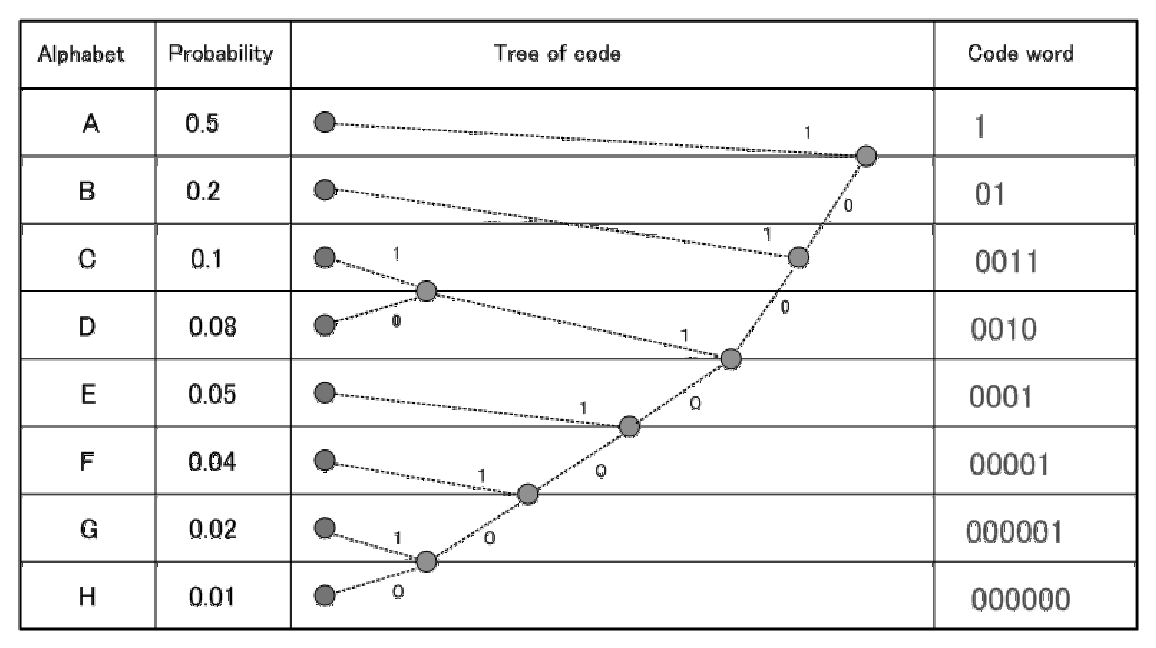
\includegraphics[width=0.8\linewidth,keepaspectratio]{fig/fig1_1.eps}
\caption{8種類の値のハフマン符号化 東邦大学メディアネットセンター 情報通信理論(佐藤 洋一)より引用} \label{fig1_1}
\end{figure}

ハフマン符号は整数の符号語長という制約のもとでは、常に最適な符号を構成できるという特徴がある。(実数の符号語長を許す場合には、レンジ符号などより高効率なものがある。)これは\textbf{シャノンの情報源符号化定理}\index{しゃのんのじょうほうげんふごうかていり@シャノンの情報源符号化定理}と呼ばれる定理により説明できる\footnote{数学的な取り扱いがやや高度であるため、本書では示さない。ここでは「圧縮できる限界を示した定理」と考えれば良い}。

\subsection{辞書式(ユニバーサル)符号}
データにおいて値が無秩序に並んでいることは少なく、なんらかの関連性があるものである。データ値の並び方のパターンを抽出し、そこに元よりも短いコードを振って出力することでデータの情報量を減らすことができる。この手法を\textbf{辞書式符号}\index{じしょしきふごう@辞書式符号}または\textbf{ユニバーサル符号}\index{ゆにばーさるふごう@ユニバーサル符号}と呼び\footnote{エントロピー符号に出てくる(整数の)ユニバーサル符号とは別の意味であるので注意。英語でも、整数の方はuniversal code、辞書式の方はuniversal source codingと名称が異なる。整数の方のユニバーサル符号とは、大きい数のほうが出現頻度が低い分布において効率的に(最適な符号化と同程度のオーダーで)符号化可能な手法の総称である。}、次のような種類がある。
\begin{itembox}[l]{ユニバーサル符号の例}
\begin{multicols}{2}
\begin{itemize}
\item バイト対符号化(BPE)
\item ランレングス(RLE)
\item LZ78
\item Deflate
\end{itemize}
\end{multicols}
\end{itembox}

以下、この内の何種類かを見ていこう。

\subsubsection{バイト対符号化(BPE)}
\textbf{バイト対符号化}\index{ばいとついふごうか@バイト対符号化}(Byte Pair Encoding)は、2バイト(2文字)の複数個の塊を辞書にする圧縮方法である。例えば、日本語で「ふらふらとふらつく」という文を考えてみよう。この文には「ふら」という文字列が3度出てくる。そこで、この2文字を仮にAに変えると「AAとAつく」と文字列がずいぶん短くなる。

このように、2文字の同一の文字列があるときこれを使われていない別のバイトに置き換えていく(再帰的に適用する)ことで、文字列をより短くできる。そして、置き換えた一覧(辞書)とともに送付することでバイト列を圧縮する。圧縮には時間がかかるが、展開はすぐにできるため、受信側が非力な機器である際に利用される手法である。

\subsubsection{LZ78}
\textbf{LZ78}\index{LZ78}は読み込んだ記号列から動的に辞書を作成して、それをもとに入力記号列を置き換えていく\textbf{動的辞書法}\index{どうてきじしょほう@動的辞書法}とも呼ばれる圧縮法である。先に示したBPEと違い、辞書を別途送ることなくデータを圧縮する。

この圧縮手順は次のようになる。
\begin{enumerate}
\item 辞書を空にし、コード値の最大を0とする。
\item データ列を走査し、データパターンが辞書に存在するか調べる。辞書に存在した場合はそのコード値を出力する。なければ、コード値0を出力する。
\item コード化を行ったデータパターンの次のデータ1つをそのまま出力する。
\item 前項・前々項で出力したデータについて、コード値を辞書の値に置き換えたデータを、新データパターンとして辞書に登録する。このときのコード値は、コード値の最大+1とする。
\item データ終端に至るまで、上記の2~4項を繰り返す。
\end{enumerate}

わかりづらいので、AAABBBAAABBBBAAAという文字列を圧縮することを考えてみよう。
\begin{enumerate}
\item 最初、辞書は空である。データ列を最初から見ていったときのパターンはAである。Aというパターンは辞書にないから、コード値0とその次のデータ(A)を出力し、辞書にはコード値1としてAを出力する。
\begin{verbatim}
文字列:A AABBBAAABBBBAAA
出力:0A
辞書: 0-(空),1-A
\end{verbatim}
\item 2文字目はAであるので、\verb|1-A|に合致する。このため、コード値1とその次のデータ(A)を出力し、辞書にはコード値2としてAAを出力する。これにより、3文字目のAまでが表されたことになる。
\begin{verbatim}
文字列:AAA BBBAAABBBBAAA
出力:0A1A
辞書: 0-(空),1-A,2-AA
\end{verbatim}
\item 4〜6文字目についても同様に行う。
\begin{verbatim}
文字列:AAABBB AAABBBBAAA
出力:0A1A0B3B
辞書: 0-(空),1-A,2-AA,3-B,4-BB
\end{verbatim}
\item 7文字目〜9文字目は、コード値2のAAにAをつけたものであるから、2Aとする。2Aに対応するAAAを辞書に登録。
\begin{verbatim}
文字列:AAABBBAAA BBBBAAA
出力:0A1A0B3B2A
辞書: 0-(空),1-A,2-AA,3-B,4-BB,5-AAA
\end{verbatim}
\item 10文字目〜12文字目は、コード値4のBBにBをつけたものであるから、2Bとする。2Bに対応するBBBを辞書に登録。
\begin{verbatim}
文字列:AAABBBAAABBB BAAA
出力:0A1A0B3B2A4B
辞書: 0-(空),1-A,2-AA,3-B,4-BB,5-AAA,6-BBB
\end{verbatim}
\item 以下、同様に繰り返す。
\begin{verbatim}
文字列:AAABBBAAABBBBAAA
出力:0A1A0B3B2A4B3A2(空)
辞書: 0-(空),1-A,2-AA,3-B,4-BB,5-AAA,6-BBB,7-BA,8-AA(空)
\end{verbatim}
\end{enumerate}

出力のデータはもとのデータより短くなっており、また出力内容から辞書を作成しつつ解凍することができるので、辞書を別途送る必要がない。これが動的辞書法と言われるゆえんである。なお、この例ではあまり長い例がないため圧縮効果が低いが、実際には辞書に長いデータが入って同じデータが頻出する場合などより効果的な圧縮となる。

またこの手法は、記号列の長さを増して部分列に分解していくことから、\textbf{増分分解法}\index{ぞうぶんぶんかいほう@増分分解法}とも呼ばれる。ユニバーサル符号の代表的な手法である。

\subsubsection{ランレングス(RLE)}
\textbf{ランレングス}\index{らんれんぐす@ランレングス}(Run Length Encoding)あるいは\textbf{連長圧縮}\index{れんちょうあっしゅく@連長圧縮|see{ランレングス}}は、同一のデータが複数続いているとき、その個数とデータで表現することにより全体の長さを短くする方法である。例えば、"AAAAAAABBBBB"というデータがあったとき、"Aが7個、Bが5個"の意味で"7A5B"とすると文字列が短くなる。これは特に、データの種類が少なく、また連続している可能性が高い場合に大きな効果を発揮する。とりわけ、白黒のファクシミリでは、白か黒かの2値であることと、よほど細かい市松のような状況でない限りは白・黒の連続性が高いと考えられることから、ランレングスがよく利用される。

\subsection{差分(デルタ)圧縮}
符号の圧縮の多くは、先に挙げたエントロピー符号または辞書式符号に分類される。しかし、その双方に分類されない(というより分類の前処理にあたる)のがここで扱う\textbf{差分圧縮}\index{さぶんあっしゅく@差分圧縮}または\textbf{デルタ圧縮}\index{でるたあっしゅく@デルタ圧縮}である。この方式は、通信よりも寧ろデータのバックアップなどによく用いられる。

定期的にシステムやデータのバックアップを取る場合を考える。その期間にもよるが、毎回全てのデータを上書きする必要はないことが多い。期間が短いほどその変化は少ないだろう。そこで現行と以前のあるバックアップ時との差分を用意し、これを保存しておく。このように、ある完全なデータを一つ用意した上で、そこからの差分を用いて圧縮するのがこの差分圧縮である。性質上、前述のエントロピー符号や辞書式符号と併用することができる。特に、差分データについては"差分なし"あるいは"僅かな差分"の部分が大半を占めることが多いため、これらに短い符号を割り当てることにより圧縮効率が高まると期待できるのである。

この例ではバックアップを出したが、関連性のある複数のデータであれば同様の効果が期待できる。現実にも定点観測のデータやソフトウェアのアップデートなどでこの手法が利用されている。

\section*{演習問題}
\begin{problems}
\item 古いゲームにおいては、容量の制約から16bitの整数型などを採用せざるを得なかった。そのため、例えば(0以下の場合は0以下になった時の処理が必要となる)体力などの数値は32768が最大となっていた(現実には、これを3〜4データ用意するなどして増強を図っていた)。ところが、この最大値は2の補数表現を採用した16bit符号付き整数型の最大値と1異なる。内部上の表現は確かに2の補数表現で間違いなく、処理によってこの違いが生じているのだが、どのような処理をしていると考えられるか説明せよ。 

\item データの種類数と、各データの出現比率が与えられるとき、そのハフマン符号化の例と、その際の平均符号長を出力するプログラムを作成せよ。例えば、4種のデータが表\ref{table1_5}のような比率で入力される場合、平均符号長は1.75となる。
\begin{table}[h]
\centering
\caption{ハフマン符号化を考えるデータ例}\label{table1_5}
\begin{tabular}{|c||c|c|c|c|}\hline
データ種別 & A & B & C & D \\ \hline
出現頻度 & 4 & 2 & 1 & 1 \\ \hline
符号例 & 0 & 10 & 110 & 111 \\ \hline
\end{tabular}
\end{table}
なお、簡単のために出現頻度は正整数値で、その合計は50000を超えないものとして良い。

\item 浮動小数点数の配列を圧縮して送りたい場合、単純なランレングスでは効果が出づらい。そこで、各値の同一ビットのみを集めてランレングスをかけ、これを順に記すことで圧縮することを考える。すなわち、1ビット目のランレングス情報、2ビット目のランレングス情報…と書かれたデータを作成して圧縮するのである。この手法について以下の問いに答えよ。
\begin{enumerate}
\item 浮動小数点数の配列にどのような傾向があるときにこの圧縮は効果的か。
\item 整数や文字の配列の場合、このように同一ビットのみを集めた圧縮は効果的と言えるか。データの特性とともに考えてみよ。
\end{enumerate}

\end{problems}
